\section{Diagrammes de classes détaillé}

\begin{figure}[H] 
    \centering
    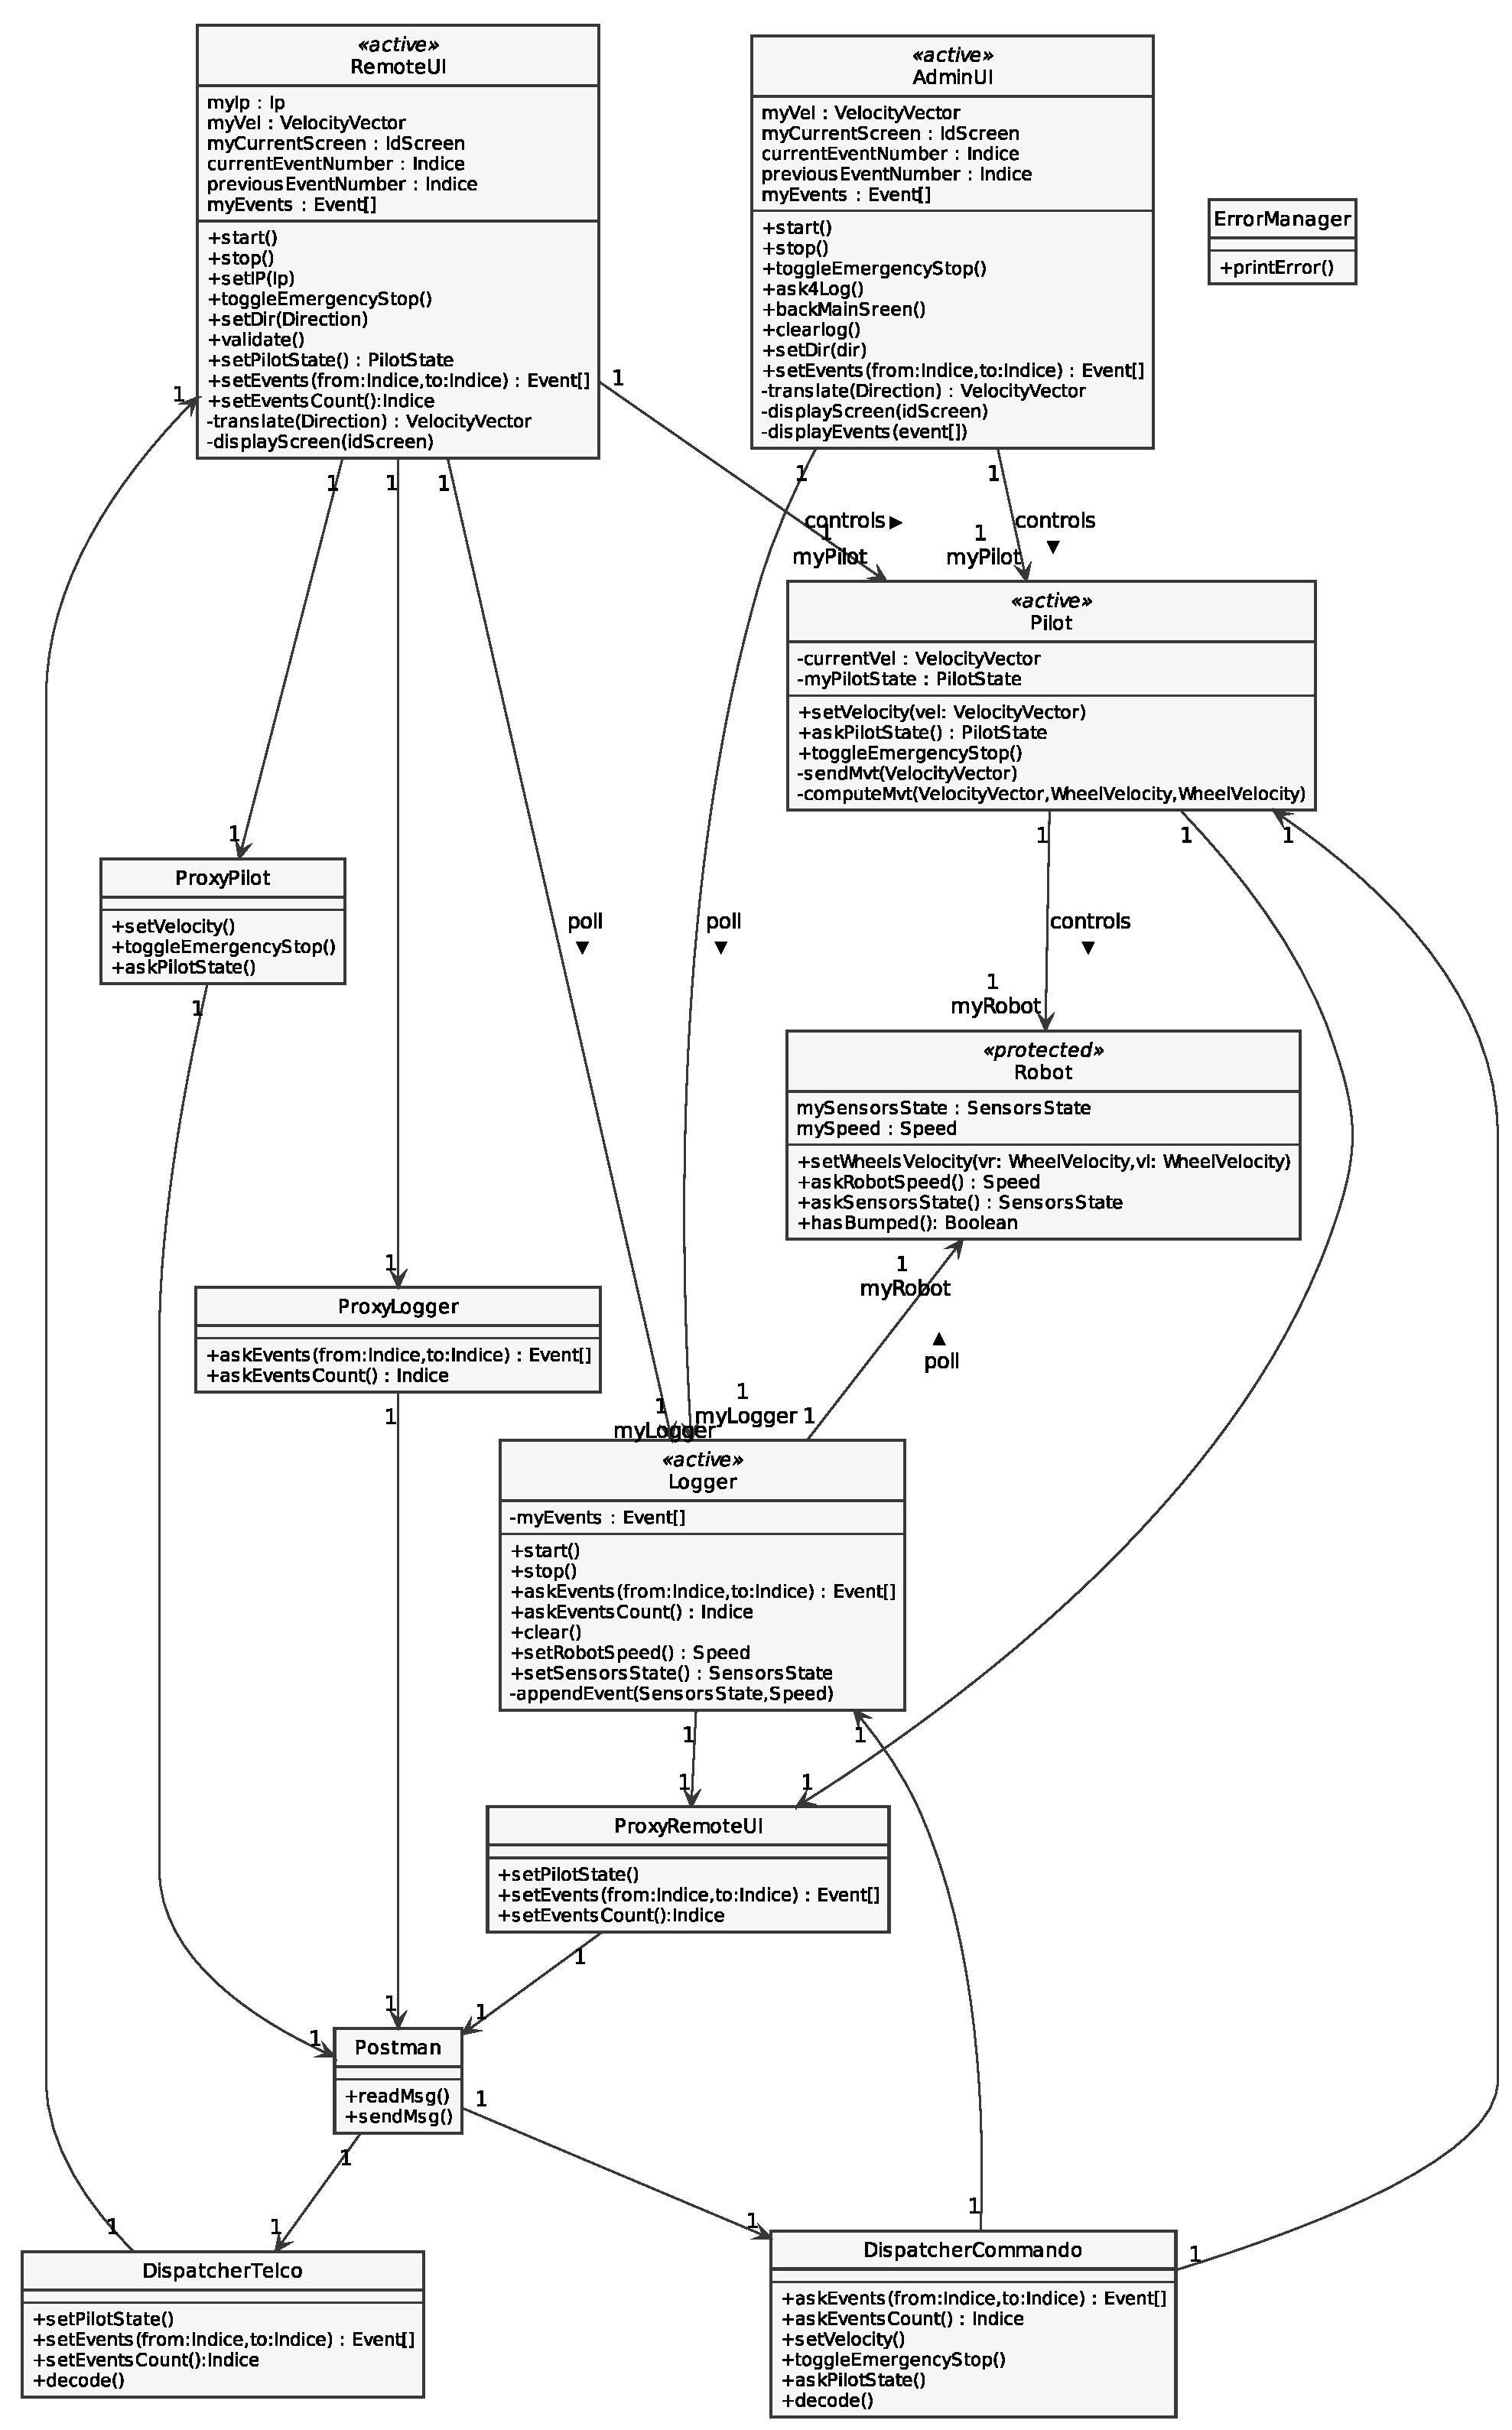
\includegraphics[width=\linewidth]{img/diagrammeClasses.eps}
    \caption{Diagramme des classes détaillé}
\end{figure}

\subsection{Comportement de Pilot}

\begin{figure}[H] 
    \centering
    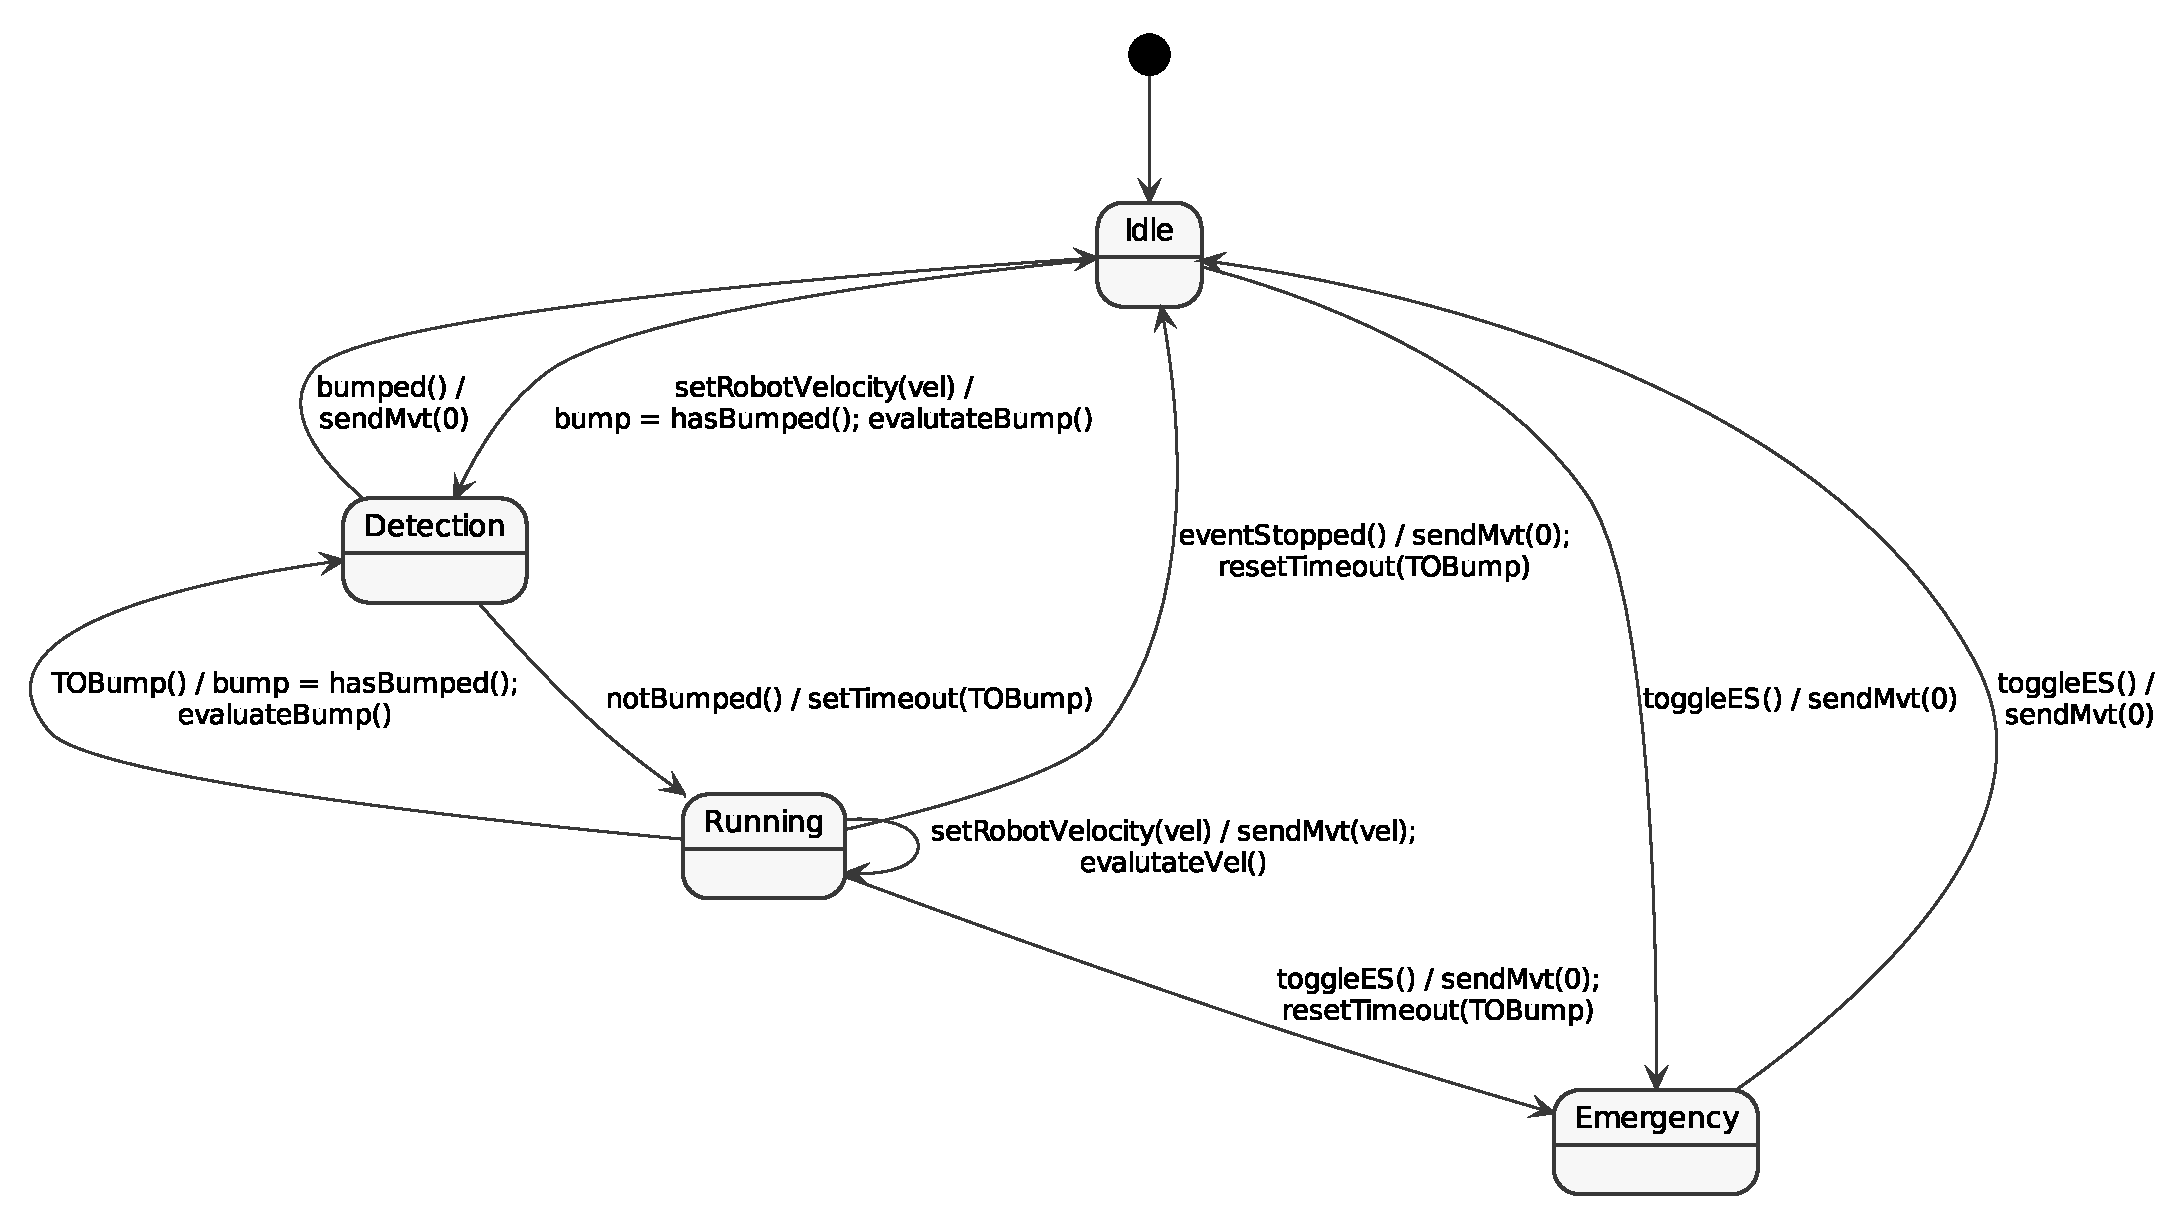
\includegraphics[width=\linewidth]{img/maePilot.eps}
    \caption{Machine à états de Pilot}
\end{figure}

Contrairement à la machine à états fournie, notre objet Pilot effecture une première détection dès le passage de Idle à Running.
Cela corrige une erreur qui permettait au robot de bouger pendant la durée du TOBump même lors de la présence d'un bump.

